\chapter{Správa dat v architektuře mikroslužeb}\label{ch:msa-data}

\chaptersummary{
   \begin{ul}
      \item způsoby integrace datových zdrojů do \g{MSA},
      \item spojování dat napříč mikroslužbami,
      \item transakční zpracování napříč mikroslužbami.
   \end{ul}
}

Databáze jako datový zdroj je jednim z možných řešení pro persistentní ukládání dat s případným následným zpracováním.
Daná kapitola je věnována především dvěma návrhovým vzorům pro organizaci dat v relačních databázích dodržujících \g{ACID} vlastnosti a spolupráci mikroslužeb pro vyhodnocování pokročilých klientských požadavků.
Popisované databázové organizace dat se obecně nemusí týkat pouze architektury mikroslužeb, ale nachází zde svoje přímé uplatnění.



\section{Typy organizace zdrojů}\label{sec:msa-db-as-data-source}

V jednoduché monolitní architektuře využití relační databáze může být zcela přímočaré – jeden monolit se připojuje k jedné databázi, která spravuje veškerá potřebná data.
Mikroslužby však představují separaci na jednotlivé částí dle zvolené dekompozice a intuitivně přináší i myšlenku dělení původně jednoho datového zdroje na obdobně dekomponované celky.
Ná základě této uvahy můžeme definovat dva návrhové vzory pro organizaci dat:

\begin{dl}
   \item [Sdílená databáze (ShDB)] – jedna instance databáze je plně přístupna pro všechny připojemé mikroslužby~\cite{shareddb}.
   \item [Databáze pro každou službu (DBpS)] – každá deklarovaná mikroslužba používá vlastní databázi (nebo schémata), do které má výhradní přistup~\cite{dbperservice}.
   V takovém případě se samozřejmě může jednat i o fyzicky samostatné databázové servery.
\end{dl}

Oba přístupy mají svoje využití dle poskytovaných vlastností.



\subsection{Sdílená databáze}\label{subsec:shared-db}

Sdílená databáze poskytuje všechna svoje úložiště všem mikroslužbám, možná realizace je znázorněna na obrázku~\ref{fig:db-shared}. \g{ACID} vlastnosti zde jsou řízeny databází a logicky se ničím neliší od komunikací s monolitickou aplikací.

\begin{figure}[htbp]
   \centering
   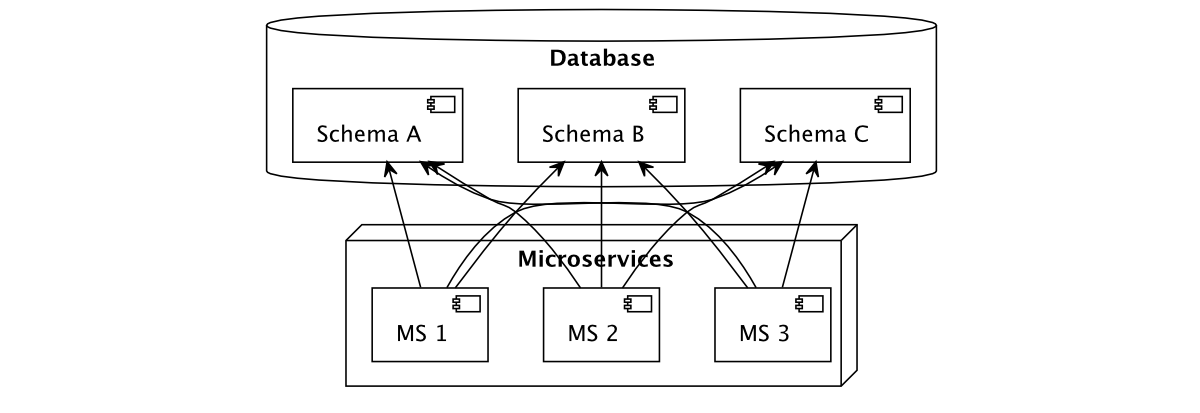
\includegraphics[max width=\textwidth]{assets/db-shared}
   \caption{Architektura sdílené databáze}\label{fig:db-shared}
\end{figure}

\textbf{Výhody}
\begin{ul}
   \item Typické použití \g{ACID} pro provádění transakcí~\cite{shareddb}.
   \item Správa jedné databáze je jednodušší~\cite{shareddb}.
\end{ul}

\textbf{Nevýhody}
\begin{ul}
   \item Databázové migrace se netýkají pouze jedné mikroslužby, ale všech zároveň, musí se vyčlenit místo pro jejich uchovávání.
   \item V případě jakékoliv změny struktury databáze je třeba změnit a otestovat všechny mikroslužby~\cite{shareddb}.
   \item Jednotná databáze nemusí vyhovovat potřebám všech mikroslužeb~\cite{shareddb}.
\end{ul}



\subsection{Databáze pro každou službu}\label{subsec:msa-db-per-service}

V případě vyčlenění jednoho schématu, či celé databáze pro každou mikroslužbu, můžeme mluvit o druhým typu struktury využití relačních databází, možná realizace je zázorněna na obrázku~\ref{fig:db-per-micro}.

\begin{figure}[htbp]
   \centering
   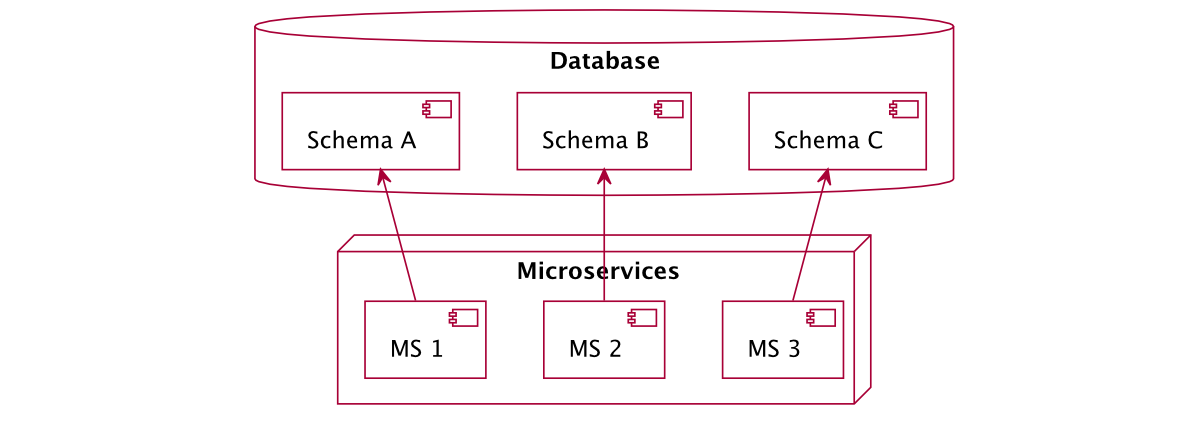
\includegraphics[max width=\textwidth]{assets/db-per-micro}
   \caption{Architektura databází (schémat) pro každou službu}\label{fig:db-per-micro}
\end{figure}



\textbf{Výhody}
\begin{ul}
   \item Zmenšení provázanosti mikroslužeb a dat, jež jsou využívány – lepší správa migrací a jiných změn~\cite{dbperservice}.
   \item Lepší možnosti škálování a volby databáze – mikroslužbě je možné poskytnout takové prostředí, které bude nejvhodnější~\cite{dbperservice}.
\end{ul}

\textbf{Nevýhody}
\begin{ul}
   \item Problém se spojováním dat z více úložiští – nelze například provádět \h{JOIN}, párovat dle cizího klíče s kontrolou integritního omezení~\cite{dbperservice}.
   \item Problém s transakčním zpracováním – transakční operace nad několika databázemi nelze jednoduše provádět a je lepší se jim úplně vyhýbat~\cite{dbperservice}.
   \item Komplikovaná správa a konfigurace většího počtu databází~\cite{dbperservice}.
\end{ul}

Nevýhody databází rozdělených dle mikroslužeb lze řešit s pomocí některých návrhových vzorů, jsou ve stručnosti popsány v následujích podkapitolách.



\section{Spojování dat mezi mikroslužbami}\label{sec:msa-db-join}
Jako jeden z možných požadavků v rámci \g{MSA} je spojení dat mezi tabulkami, což v rámci oddělených služeb znamená netriviální úkol.
Jako typický příklad lze vzít existenci tabulek \h{users} (osobní informace) a \h{payments} (částky a primárního klíče z \h{users}), jež se nachází v oddělených databázích, ze kterých je třeba získat seznam transakcí všech lidí s určitým věkem.
Spojení v tomto případě nemůžeme nechávat na databázi, situace se může řešit API kompozicí nebo \g{CQRS}.



\subsection{API kompozice}\label{subsec:msa-db-aggregate-api}

API kompozice je řešení bez využití dodatečných systémů.
Spočívá v logickém rozdělení původního dotazu na parciální dle jednotlivých mikroslužeb a následným provedení například simulace \h{JOIN} operace v aplikaci (v paměti)~\cite{apicomposition}.
Schématicky je tato operace znázorněna na obrázku~\ref{fig:api-composition}.
Samozřejmě takové řešení může přinést větší nároky na paměť v případě pracování obrovských datových celků.


\begin{figure}[htbp]
   \centering
   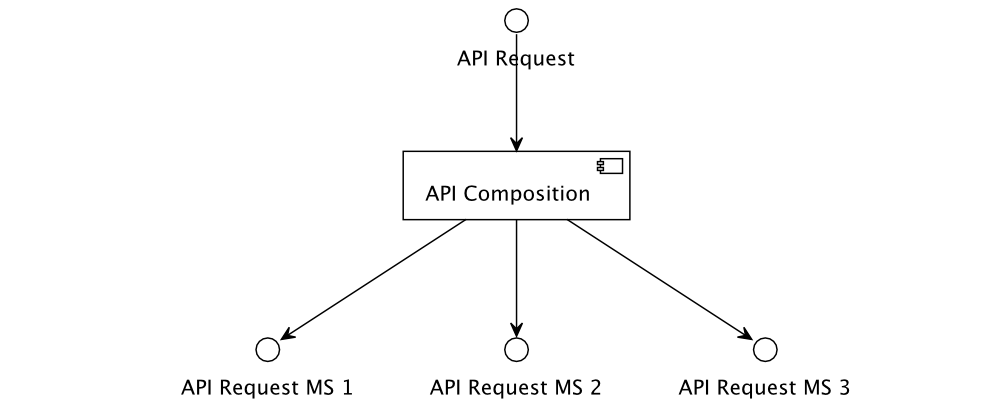
\includegraphics[max width=\textwidth]{assets/api-composition}
   \caption{Schéma vzoru API kompozice}\label{fig:api-composition}
\end{figure}



\subsection{CQRS}\label{subsec:msa-db-aggregate-cqrs}

\g{CQRS} vzor může soužit jako řešení s nedostatkem pamětí, případně výkonu, které vzniká operováním s daty v aplikaci.
Absence možnosti spojení je tu řešena dodatečnou, eventuálně konzistentní databází~\cite{msachris}, viz obrázek~\ref{fig:cqrs}.
Slouží jako zdroj dat pro čtení, který obsahuje kopie databázový pohled na strukturu dat potřebou pro provední klientského dotazu.
Existující relační databáze fungují jako persistentní úložiště pro zápis, uchovávají si informace a posílají potřebnou kopii dat do databáze pro čtení~\cite{cqrs}.
Takovým způsobem se vytváří databáze, která obsahuje minimální potřebné množeství informací například pro operaci \h{JOIN} bez nutnosti přístupu s databázím mikroslužeb.
Samozřejmě je nutné zajistit eventuální konzistenci takové databáze, aby nedocházelo ke ztrátě dat~\cite{cqrs}.



\begin{figure}[htbp]
   \centering
   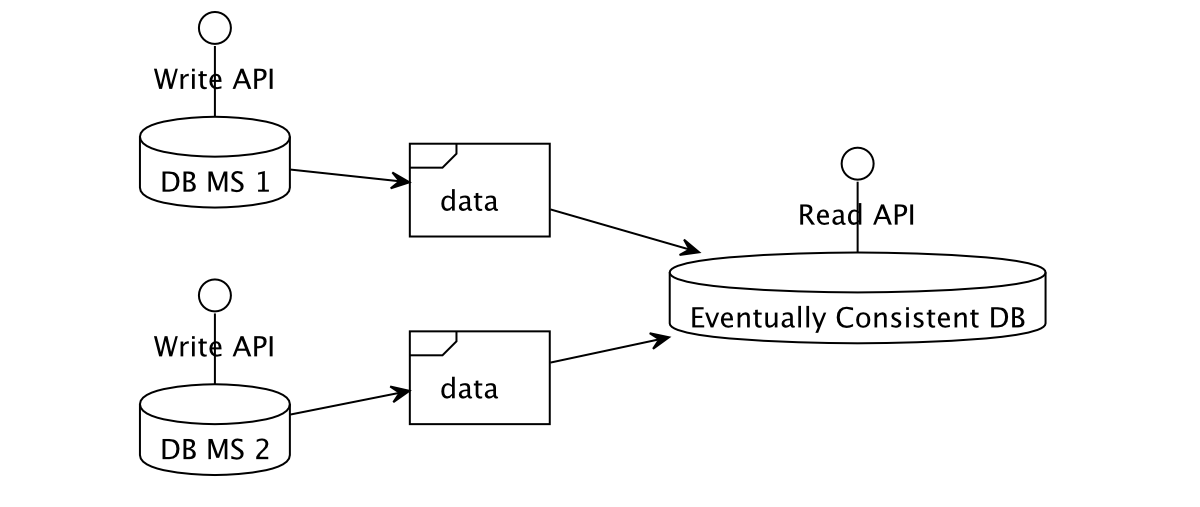
\includegraphics[max width=\textwidth]{assets/cqrs}
   \caption{Zjednodušený model CQRS vzoru}\label{fig:cqrs}
\end{figure}



\section{Transakční zpracování zápisů}\label{sec:msa-db-transaction}
V relačních databázích jsou transakce chápány jako logické celky pro čtení nebo zápis informací, které dodržují \g{ACID} vlastnosti~\cite{dbtransactions}.
Pokud existuje víc datových zdrojů a je třeba provést požadavek na zápis, jenž musí ovlivnit data v několika databázích, tak nastává problém neizolovanosti zápisu~\cite{msachris}.
Během zpracování požadavku každá mikroslužba na základě komunikace dostane příkaz o zápisu a provede je v souladu s \g{ACID}, pokud však alespoň jedna z dílčích částí nebude úspěšná, tak \h{ROLLBACK} transakce bude uskutečněn pouze v chybné.


Takové situace se mohou řešit například s pomocí ditribuovaných transakcí, nebo návrhového vzoru \h{sága}\footnote{Anglicky též \enquote{saga}}~\cite{msachris}.

Distribuované transakce (DT) jsou metodou, která propojuje víc datových zdrojů (v tomto případě databází), zpravidla stejného typu, a během zpracování transakce zajištuje \g{ACID} zápis napříč databázemi~\cite{distributedtransactions}.
Dá se říct, že DT odstraňuje jedné transakci omezení z hlediska počtu databází prostřednicvím vhodné konfigurace~\cite{distributedtransactionsintegration}.

Sága je realizována na straně serverové aplikace, jedná se o kontrolovanou sekvenci souštění lokálních transakcí.
Každá dílčí transakce po svém provedení posílá zprávu nebo vyvolává událost, jež spouští další transakci dle určeného pořadí.
Pokud jedna z lokálních transakcí skončí chybou, pak obdobným způsobem se spouští sekvence zpětných transakcí všech předchozích úprav~\cite{saga}.
Tímto je docílena chybějící izolace napříč databázemi.
Příklad takové struktury lze vidět na obrázku~\ref{fig:saga}.



\begin{figure}[htbp]
   \centering
   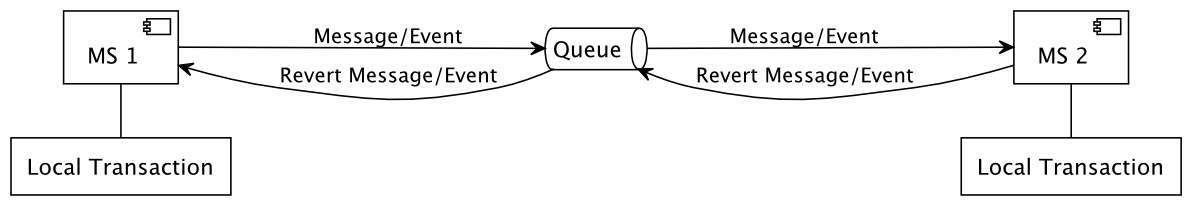
\includegraphics[max width=\textwidth]{assets/saga}
   \caption{Koncept transakčního zpracování v ságách}\label{fig:saga}
\end{figure}

%\subsection{Sága – choreografie}\label{subsec:msa-db-transaction-saga-choreography}
%\subsection{Sága – orchestrace}\label{subsec:msa-db-transaction-saga-orchestration}
